\documentclass[10pt,spanish,a4paper,oneside]{article}
\usepackage{lmodern}
\usepackage{amssymb,amsmath}
\usepackage{ifxetex,ifluatex}
\usepackage{fixltx2e} % provides \textsubscript
\ifnum 0\ifxetex 1\fi\ifluatex 1\fi=0 % if pdftex
  \usepackage[T1]{fontenc}
  \usepackage[utf8]{inputenc}
\else % if luatex or xelatex
  \ifxetex
    \usepackage{mathspec}
  \else
    \usepackage{fontspec}
  \fi
  \defaultfontfeatures{Ligatures=TeX,Scale=MatchLowercase}
    \setmainfont[]{Calibri}
    \setmonofont[Mapping=tex-ansi,Scale=0.7]{Source Code Pro}
\fi
% use upquote if available, for straight quotes in verbatim environments
\IfFileExists{upquote.sty}{\usepackage{upquote}}{}
% use microtype if available
\IfFileExists{microtype.sty}{%
\usepackage{microtype}
\UseMicrotypeSet[protrusion]{basicmath} % disable protrusion for tt fonts
}{}
\usepackage[tmargin = 2 cm,bmargin= 3 cm,lmargin= 2.5 cm,rmargin= 2 cm]{geometry}
\usepackage{hyperref}
\PassOptionsToPackage{usenames,dvipsnames}{color} % color is loaded by hyperref
\hypersetup{unicode=true,
            pdftitle={Plantilla para informe en pdf},
            pdfauthor={FVB},
            colorlinks=true,
            linkcolor=blue,
            citecolor=red,
            urlcolor=blue,
            breaklinks=true}
\urlstyle{same}  % don't use monospace font for urls
\ifnum 0\ifxetex 1\fi\ifluatex 1\fi=0 % if pdftex
  \usepackage[shorthands=off,main=spanish]{babel}
\else
  \usepackage{polyglossia}
  \setmainlanguage[]{spanish}
\fi
\usepackage{natbib}
\bibliographystyle{apalike}
\usepackage{color}
\usepackage{fancyvrb}
\newcommand{\VerbBar}{|}
\newcommand{\VERB}{\Verb[commandchars=\\\{\}]}
\DefineVerbatimEnvironment{Highlighting}{Verbatim}{commandchars=\\\{\}}
% Add ',fontsize=\small' for more characters per line
\usepackage{framed}
\definecolor{shadecolor}{RGB}{248,248,248}
\newenvironment{Shaded}{\begin{snugshade}}{\end{snugshade}}
\newcommand{\KeywordTok}[1]{\textcolor[rgb]{0.27,0.27,0.27}{\textbf{{#1}}}}
\newcommand{\DataTypeTok}[1]{\textcolor[rgb]{0.27,0.27,0.27}{{#1}}}
\newcommand{\DecValTok}[1]{\textcolor[rgb]{0.06,0.06,0.06}{{#1}}}
\newcommand{\BaseNTok}[1]{\textcolor[rgb]{0.06,0.06,0.06}{{#1}}}
\newcommand{\FloatTok}[1]{\textcolor[rgb]{0.06,0.06,0.06}{{#1}}}
\newcommand{\ConstantTok}[1]{\textcolor[rgb]{0,0,0}{{#1}}}
\newcommand{\CharTok}[1]{\textcolor[rgb]{0.5,0.5,0.5}{{#1}}}
\newcommand{\SpecialCharTok}[1]{\textcolor[rgb]{0,0,0}{{#1}}}
\newcommand{\StringTok}[1]{\textcolor[rgb]{0.5,0.5,0.5}{{#1}}}
\newcommand{\VerbatimStringTok}[1]{\textcolor[rgb]{0.5,0.5,0.5}{{#1}}}
\newcommand{\SpecialStringTok}[1]{\textcolor[rgb]{0.5,0.5,0.5}{{#1}}}
\newcommand{\ImportTok}[1]{{#1}}
\newcommand{\CommentTok}[1]{\textcolor[rgb]{0.37,0.37,0.37}{\textit{{#1}}}}
\newcommand{\DocumentationTok}[1]{\textcolor[rgb]{0.37,0.37,0.37}{\textbf{\textit{{#1}}}}}
\newcommand{\AnnotationTok}[1]{\textcolor[rgb]{0.37,0.37,0.37}{\textbf{\textit{{#1}}}}}
\newcommand{\CommentVarTok}[1]{\textcolor[rgb]{0.37,0.37,0.37}{\textbf{\textit{{#1}}}}}
\newcommand{\OtherTok}[1]{\textcolor[rgb]{0.37,0.37,0.37}{{#1}}}
\newcommand{\FunctionTok}[1]{\textcolor[rgb]{0,0,0}{{#1}}}
\newcommand{\VariableTok}[1]{\textcolor[rgb]{0,0,0}{{#1}}}
\newcommand{\ControlFlowTok}[1]{\textcolor[rgb]{0.27,0.27,0.27}{\textbf{{#1}}}}
\newcommand{\OperatorTok}[1]{\textcolor[rgb]{0.43,0.43,0.43}{\textbf{{#1}}}}
\newcommand{\BuiltInTok}[1]{{#1}}
\newcommand{\ExtensionTok}[1]{{#1}}
\newcommand{\PreprocessorTok}[1]{\textcolor[rgb]{0.37,0.37,0.37}{\textit{{#1}}}}
\newcommand{\AttributeTok}[1]{\textcolor[rgb]{0.61,0.61,0.61}{{#1}}}
\newcommand{\RegionMarkerTok}[1]{{#1}}
\newcommand{\InformationTok}[1]{\textcolor[rgb]{0.37,0.37,0.37}{\textbf{\textit{{#1}}}}}
\newcommand{\WarningTok}[1]{\textcolor[rgb]{0.37,0.37,0.37}{\textbf{\textit{{#1}}}}}
\newcommand{\AlertTok}[1]{\textcolor[rgb]{0.33,0.33,0.33}{{#1}}}
\newcommand{\ErrorTok}[1]{\textcolor[rgb]{0.14,0.14,0.14}{\textbf{{#1}}}}
\newcommand{\NormalTok}[1]{{#1}}
\usepackage{longtable,booktabs}
\usepackage{graphicx,grffile}
\makeatletter
\def\maxwidth{\ifdim\Gin@nat@width>\linewidth\linewidth\else\Gin@nat@width\fi}
\def\maxheight{\ifdim\Gin@nat@height>\textheight\textheight\else\Gin@nat@height\fi}
\makeatother
% Scale images if necessary, so that they will not overflow the page
% margins by default, and it is still possible to overwrite the defaults
% using explicit options in \includegraphics[width, height, ...]{}
\setkeys{Gin}{width=\maxwidth,height=\maxheight,keepaspectratio}
\IfFileExists{parskip.sty}{%
\usepackage{parskip}
}{% else
\setlength{\parindent}{0pt}
\setlength{\parskip}{6pt plus 2pt minus 1pt}
}
\setlength{\emergencystretch}{3em}  % prevent overfull lines
\providecommand{\tightlist}{%
  \setlength{\itemsep}{0pt}\setlength{\parskip}{0pt}}
\setcounter{secnumdepth}{5}
% Redefines (sub)paragraphs to behave more like sections
\ifx\paragraph\undefined\else
\let\oldparagraph\paragraph
\renewcommand{\paragraph}[1]{\oldparagraph{#1}\mbox{}}
\fi
\ifx\subparagraph\undefined\else
\let\oldsubparagraph\subparagraph
\renewcommand{\subparagraph}[1]{\oldsubparagraph{#1}\mbox{}}
\fi

%%% Use protect on footnotes to avoid problems with footnotes in titles
\let\rmarkdownfootnote\footnote%
\def\footnote{\protect\rmarkdownfootnote}

%%% Change title format to be more compact
\usepackage{titling}

% Create subtitle command for use in maketitle
\newcommand{\subtitle}[1]{
  \posttitle{
    \begin{center}\large#1\end{center}
    }
}

\setlength{\droptitle}{-2em}
  \title{Plantilla para informe en pdf}
  \pretitle{\vspace{\droptitle}\centering\huge}
  \posttitle{\par}
  \author{FVB}
  \preauthor{\centering\large\emph}
  \postauthor{\par}
  \date{}
  \predate{}\postdate{}

\usepackage[utf8]{inputenc}
\usepackage{graphicx}
\usepackage[labelfont=bf]{caption}
\usepackage{float}
\usepackage{fancyhdr}
\usepackage{fancyheadings}
\pagestyle{fancy}
\lhead{{\scriptsize C/ Montijo, 2, 3ª planta\\ -30001 Murcia-\\Tel. 968 355 337 - Fax. 968 22 23 25\\ \textit{\scriptsize www.acuamed.es }}}
\chead{}
\rhead{
\includegraphics[height=0.1\textwidth]{logo1.jpg}}
\lfoot{\scriptsize -Informe obras- }{\scriptsize}
\cfoot{}
\rfoot{\thepage}

\let\BeginKnitrBlock\begin \let\EndKnitrBlock\end
\begin{document}
\maketitle

{
\hypersetup{linkcolor=black}
\setcounter{tocdepth}{3}
\tableofcontents
}
\pagebreak

\begin{titlepage}
    \begin{scriptsize} 
        \listoffigures
    \end{scriptsize} 
\end{titlepage}

\pagebreak

\break
\[\\*\]

\section{INSTRUCCIONES}\label{instrucciones}

Para duplicar en otro informe esta plantilla que genera un documento en
pdf tipo informe hay que realizar el siguiente proceso:

\begin{enumerate}
\def\labelenumi{\arabic{enumi}.}
\tightlist
\item
  copiar el directorio completo con todos sus archivos en otra
  ubicación.
\item
  cambiar de nombre a la nueva carpeta.
\item
  abrir RSTUDIO y abrir nuevo proyecto --\textgreater{} carpeta
  existente y seleccionar la carpeta renombrada en el punto anterior
\item
  continuar y crear nuevo proyecto en ese carpeta en una nueva sesión
\item
  RSTUDIO creará un nuevo fichero \texttt{nombre\_carpeta.Rproj} que es
  el nuevo proyecto.
\item
  modificar los ficheros de configuracion para cambiar titulos etc..

  \begin{enumerate}
  \def\labelenumii{\arabic{enumii}.}
  \tightlist
  \item
    el fichero \texttt{\_bookdown.yml} sirve para asignar el idioma y
    nombres de equivalencia
  \item
    el fichero \texttt{\_output.yml} indica el formato de salida y sus
    opciones (pdf en este caso)
  \end{enumerate}
\item
  cada fichero *.Rmd se compilará para el libro o informe final como un
  capitulo del pdf, por orden alfabetico de su nombre.
\item
  podemos añadir cuanto s*.Rmd queramos comenzando.
\item
  el fichero ìndex.Rmd`es el principal que inicia el proceso de
  complilación y en el que se pueden incluir encabezados tipo YAML como
  el título, autor etc.
\item
  una vez completo el documento o para ver la salida hay que ejecutar la
  orden siguiente en la linea de comandos de R:
  \texttt{bookdown::render\_book(\textquotesingle{}index.Rmd\textquotesingle{},\ \textquotesingle{}bookdown::pdf\_book\textquotesingle{})}
  incluso se pueden pasar ordenes como:
  \texttt{bookdown::render\_book(\textquotesingle{}index.Rmd\textquotesingle{},\ bookdown::pdf\_book(keep\_tex\ =\ TRUE))}
\end{enumerate}

\subsection{Instalación de bookdown}\label{instalacion-de-bookdown}

Para usar esta plantilla debes tener la libraría \texttt{bookdown}
instalada en R y el programa RSTUDIO.

Para instalar el paquete haremos: \texttt{install.packages("bookdown")}

\subsection{\texorpdfstring{Enlaces internos y entre documentos
\label{enlaces}}{Enlaces internos y entre documentos }}\label{enlaces-internos-y-entre-documentos}

Los enlaces internos en el mismo documento se deben hacer con formato
\(LaTeX\) y no con markdown. Ejemplos:

\begin{itemize}
\tightlist
\item
  para poner el enlace a una parte del documento debemos escribir esto
  \texttt{\textbackslash{}label\{enlaces\}} y para crear la referencia a
  dicho enlace esto otro: (ver Fig:\ref{fig_9}).
\end{itemize}

\begin{figure}[htbp]
\centering
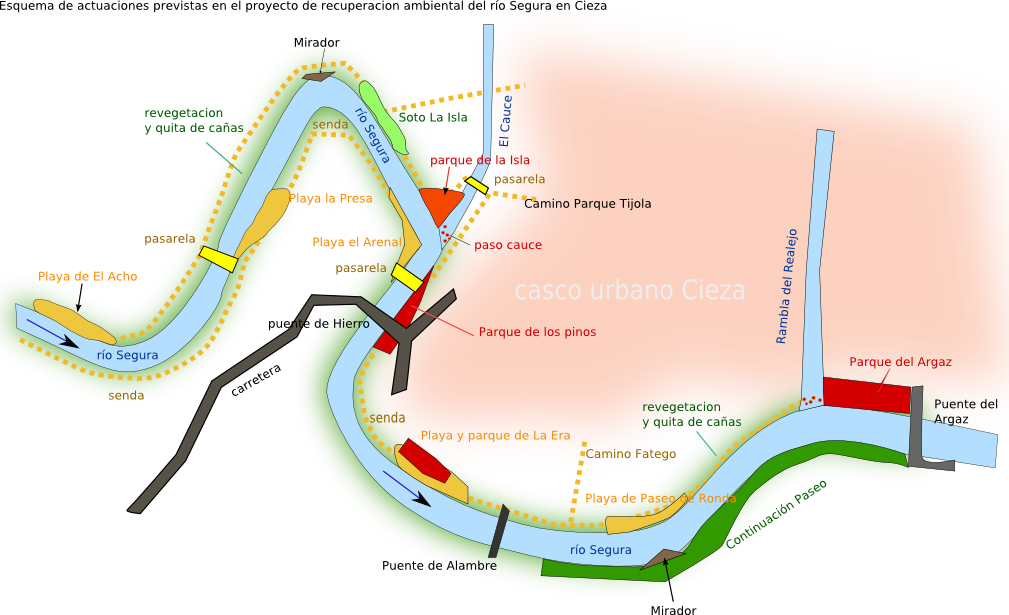
\includegraphics{imag/portada.png}
\caption{titulo figura aaa \label{fig_9}}
\end{figure}

Por ejemplo enlaces a los capitulos principales :

\begin{itemize}
\tightlist
\item
  descripcion \{\ref{des}\}
\item
  cronología \{\ref{crono}\}
\item
  bibliografía \{\ref{ref}\}
\end{itemize}

Para ir a la documentación ir a enlace \{\ref{doc}\}.

También se pueden hacer referencias a elementos como una tabla, ver los
datos en la tabla \ref{tab:aTable}) o \{\ref{tab:aTable}\}.

\begin{table}

\caption{\label{tab:aTable}See Section \ref{enlaces}.}
\centering
\begin{tabular}[t]{r|r}
\hline
speed & dist\\
\hline
4 & 2\\
\hline
4 & 10\\
\hline
7 & 4\\
\hline
7 & 22\\
\hline
8 & 16\\
\hline
\end{tabular}
\end{table}

\subsection{\texorpdfstring{Encabezado yaml
\label{yaml1}}{Encabezado yaml }}\label{encabezado-yaml}

La informacion de los tipos de cosas que se pueden poner en yml está en
\url{http://pandoc.org/MANUAL.html\#variables-for-latex}

\subsection{\texorpdfstring{Bibliografía
\label{bib}}{Bibliografía }}\label{bibliografia}

las referencias a libros que esten en la bibliografia deben meterse
primero la ficha en los ficheros de bibliografía como
\texttt{libros.bib}, y una vez esten en esa ficha basta con hacer el
siguiente enlace para que aparezcan en la pagina de referencias:

Este libro ha sido escrito en R, si quieres iniciarte en R mira
\citep{R-Fer}. Si quieres aprender Knitr lee \citep{R-knitr}

Es

\section{\texorpdfstring{DESCRIPCIÓN DE LAS OBRAS
\label{des}}{DESCRIPCIÓN DE LAS OBRAS }}\label{descripcion-de-las-obras}

\subsection{Formato}\label{formato}

hay una web que indica muy bien como usar el YAML
\url{https://bookdown.org/yihui/bookdown/publishers.html}

\subsection{tipo de letra}\label{tipo-de-letra}

Puedes elegir las letras que existan en la versionde latex local, en
principio valen todas las listadas en :

-\url{http://www.tug.dk/FontCatalogue/}

Pero muchas de ellas no estarán en el fichero sty necesario. Por ejemplo
:

\begin{itemize}
\tightlist
\item
  Chivo Light
\item
  Bookman
\item
  Garamond
\item
  Latin Modern Roman
\end{itemize}

\subsection{Proyecto de arte
dramático}\label{proyecto-de-arte-dramatico}

El proyecto consiste básicamente, en las siguientes actuaciones:

\begin{enumerate}
\def\labelenumi{\arabic{enumi}.}
\tightlist
\item
  Toma en el embalse del Talave
\item
  Túnel
\item
  Obra de salida a la rambla del Algarrobo que desemboca en la cola del
  embalse del Cenajo.
\end{enumerate}

\subsubsection{Túnel}\label{tunel}

El proyecto original consistía en la construcción de un túnel de 4,5 m
de diámetro y una longitud total de 7,5 km. Se diseñó una conducción
\textbf{a presión} en túnel capaz de desaguar 60 \(m^3/s\) desde el
embalse del Talave al embalse del Cenajo.

\subsubsection{Plazo de ejecución del
PM1}\label{plazo-de-ejecucion-del-pm1}

Para saber cómo meter fórmulas mat en los documentos se puede consultar
la web: \url{https://en.wikibooks.org/wiki/LaTeX/Mathematics}

formulas matemáticas son faciles de introducir con codigo \(LaTeX\):
\[\frac{x*x^2}{P_1 + \pi}\]

nada de esto es cierto

\subsection{graficas}\label{graficas}

\begin{Shaded}
\begin{Highlighting}[]
\KeywordTok{head}\NormalTok{(cars)}
\end{Highlighting}
\end{Shaded}

\begin{verbatim}
##   speed dist
## 1     4    2
## 2     4   10
## 3     7    4
## 4     7   22
## 5     8   16
## 6     9   10
\end{verbatim}

\begin{Shaded}
\begin{Highlighting}[]
\KeywordTok{with}\NormalTok{(cars, }\KeywordTok{plot}\NormalTok{(speed, dist, }\DataTypeTok{main=}\StringTok{"grafico"}\NormalTok{))}
\end{Highlighting}
\end{Shaded}

\includegraphics{01-intro_files/figure-latex/unnamed-chunk-2-1.pdf}

Esto es todo amigos

\BeginKnitrBlock{flushright}
Vilber Murcia, España
\EndKnitrBlock{flushright}

\section{\texorpdfstring{CRONOLOGÍA
\label{crono}}{CRONOLOGÍA }}\label{cronologia}

\begin{Shaded}
\begin{Highlighting}[]
\KeywordTok{boxplot}\NormalTok{(dist~speed, cars)}
\end{Highlighting}
\end{Shaded}

\includegraphics{02-crono_files/figure-latex/unnamed-chunk-1-1.pdf}

\subsection{Origen del Proyecto}\label{origen-del-proyecto}

El 10 de mayo de 1981 la Dirección General de Obras Hidráulicas del
Ministerio de Obras Públicas autorizó a la Confederación Hidrográfica
del Segura la redacción del Proyecto del Túnel Talave-Cenajo. Dicho
Proyecto fue redactado y se Aprobó técnicamente en el año 1982.

\section{\texorpdfstring{DOCUMENTOS
\label{doc}}{DOCUMENTOS }}\label{documentos}

Se aportan lo principales documentos del proyecto, ordenados según su
cronología.

\subsection{Escritos por fecha}\label{escritos-por-fecha}

este es el ouou.yml anterior:

\begin{Shaded}
\begin{Highlighting}[]
\NormalTok{bookdown::pdf_book:}
\StringTok{  }\NormalTok{includes:}
\StringTok{    }\NormalTok{template:}\StringTok{ }\NormalTok{latex/default.tex}
  \NormalTok{keep_tex:}\StringTok{ }\NormalTok{no}
  \NormalTok{toc_depth:}\StringTok{ }\DecValTok{2}
  \NormalTok{toc_unnumbered:}\StringTok{ }\NormalTok{no}
  \NormalTok{toc_appendix:}\StringTok{ }\NormalTok{yes}
\NormalTok{quote_footer:}\StringTok{ }\NormalTok{[}\StringTok{"}\CharTok{\textbackslash{}\textbackslash{}}\StringTok{VA\{"}\NormalTok{, }\StringTok{"\}\{\}"}\NormalTok{]}
\end{Highlighting}
\end{Shaded}

\subsubsection{2001}\label{section}

\section{\texorpdfstring{FOTOGRAFÍAS
\label{fotos}}{FOTOGRAFÍAS }}\label{fotografias}

Se muestran fotografías de las actuaciones, tanto durante las obras como
de las visitas realizadas en fase de explotación.

\subsection{imagenes 1}\label{imagenes-1}

\begin{Shaded}
\begin{Highlighting}[]
\NormalTok{knitr::}\KeywordTok{include_graphics}\NormalTok{(}\StringTok{"imag/20151118_095058.jpg"}\NormalTok{)}
\end{Highlighting}
\end{Shaded}

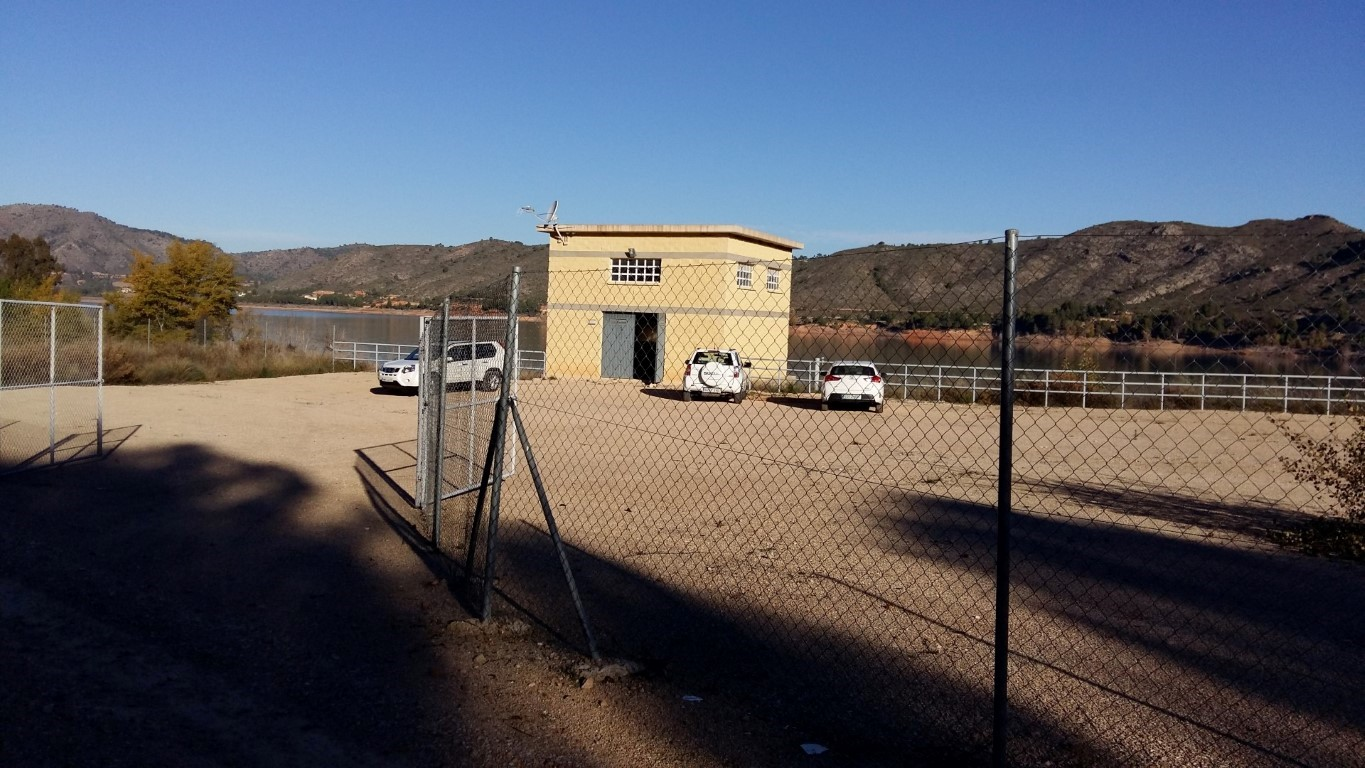
\includegraphics[width=0.3\linewidth]{imag/20151118_095058}

\subsection{imagenes 2}\label{imagenes-2}

\begin{Shaded}
\begin{Highlighting}[]
\NormalTok{knitr::}\KeywordTok{include_graphics}\NormalTok{(}\StringTok{"imag/20151118_095137.jpg"}\NormalTok{)}
\end{Highlighting}
\end{Shaded}

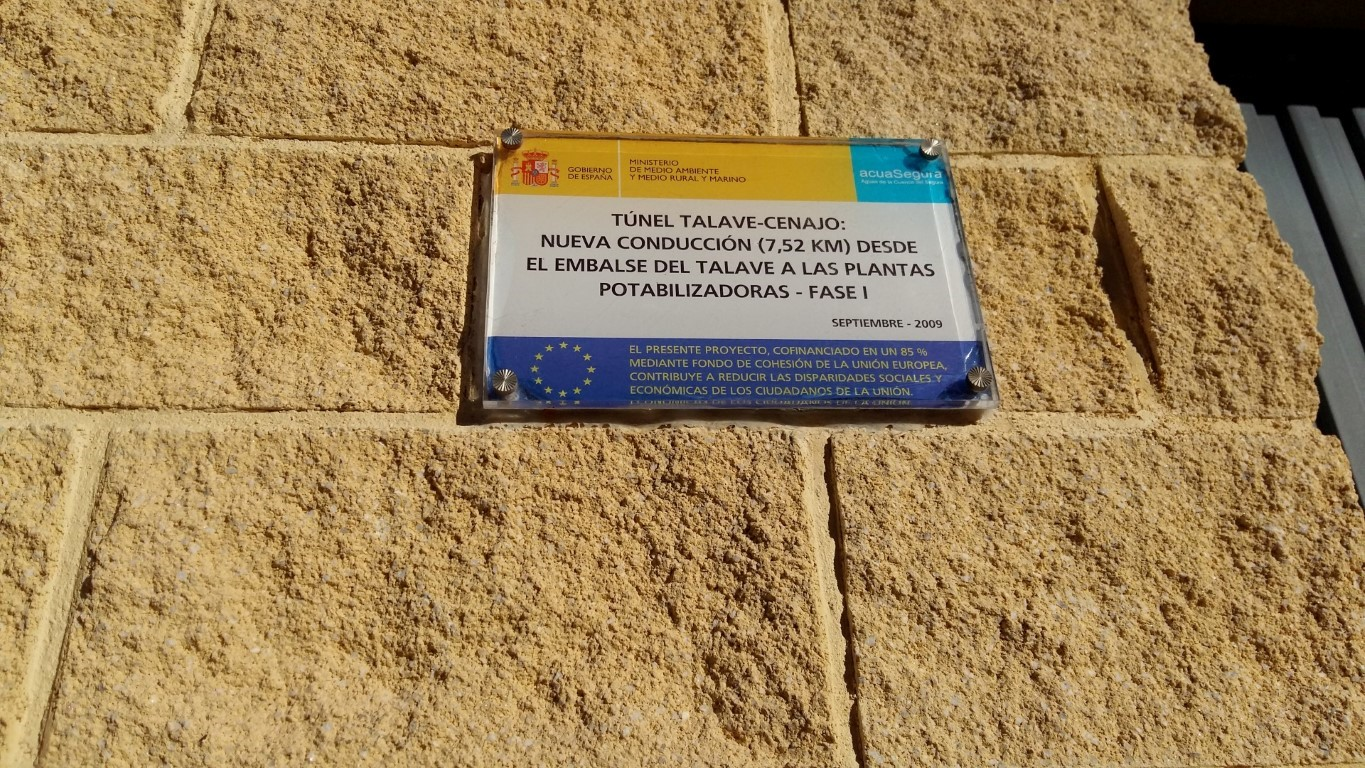
\includegraphics[width=0.5\linewidth]{imag/20151118_095137}

\subsection{OTROS TRUCOS}\label{otros-trucos}

Insertar todas las imagenes de una carpeta, se usa el ancho para
configurar la matriz de imagenespor ejemplo poniendo
\texttt{out.width="30\%"}

\begin{Shaded}
\begin{Highlighting}[]
\CommentTok{# pintamos todas las imagenes}
\KeywordTok{library}\NormalTok{(knitr)}
\NormalTok{myimages<-}\KeywordTok{list.files}\NormalTok{(}\StringTok{"imag/"}\NormalTok{, }\DataTypeTok{pattern =} \StringTok{".jpg"}\NormalTok{, }\DataTypeTok{full.names =} \OtherTok{TRUE}\NormalTok{)}
\KeywordTok{include_graphics}\NormalTok{(myimages)}
\end{Highlighting}
\end{Shaded}

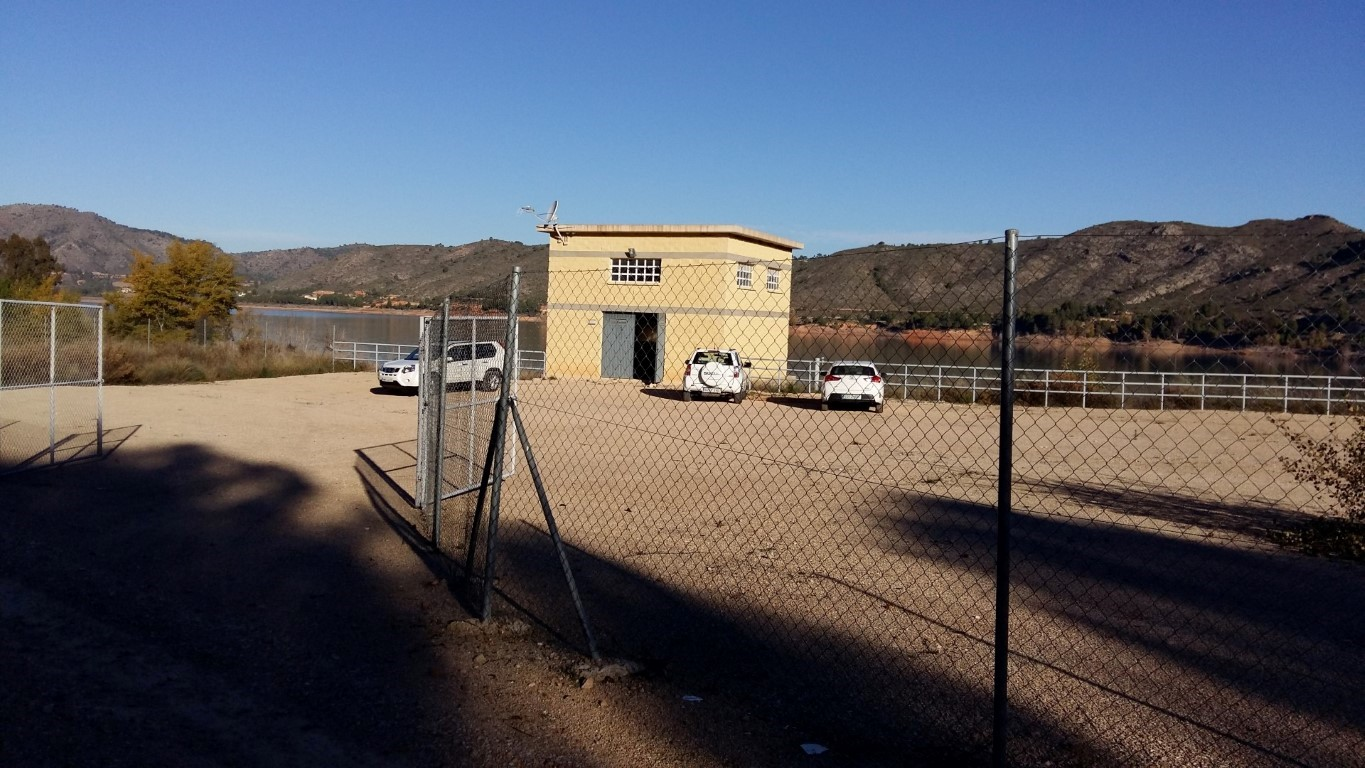
\includegraphics[width=0.3\linewidth]{imag/20151118_095058}
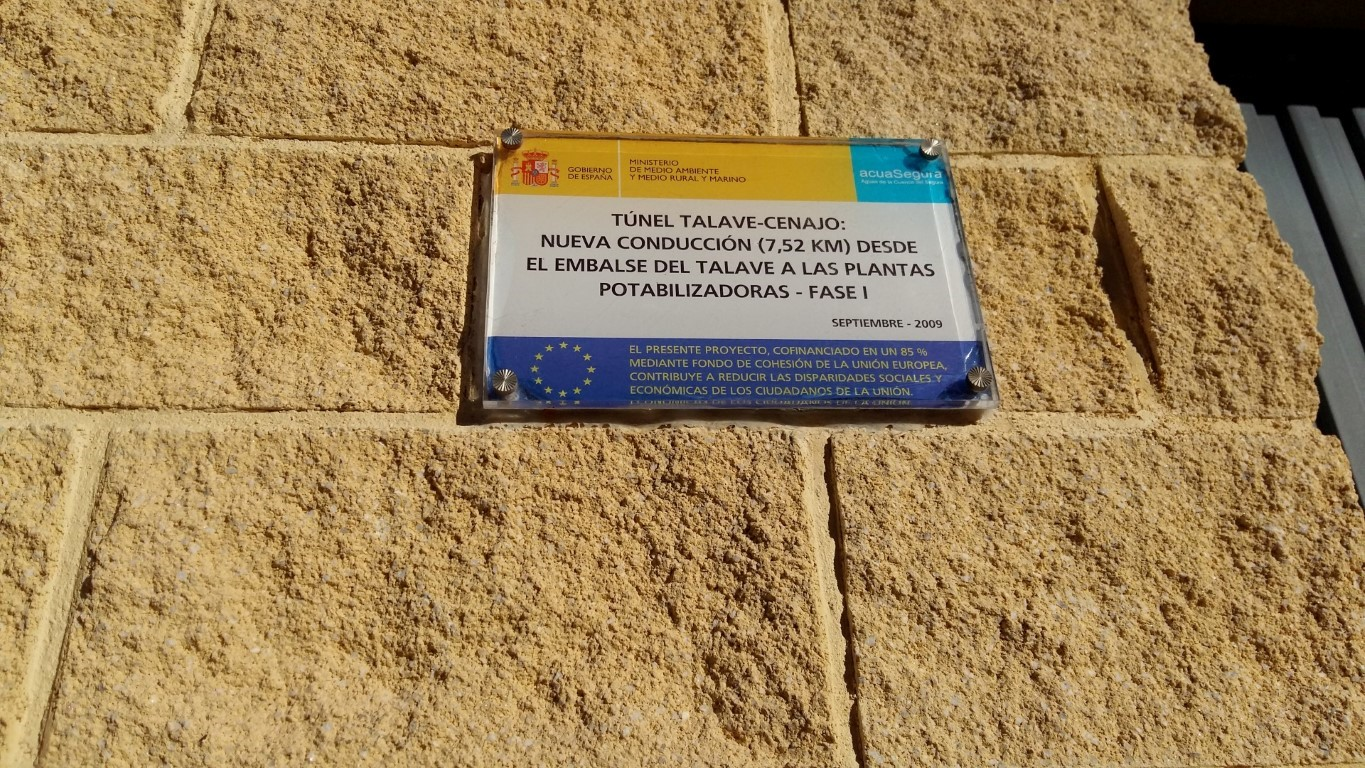
\includegraphics[width=0.3\linewidth]{imag/20151118_095137}
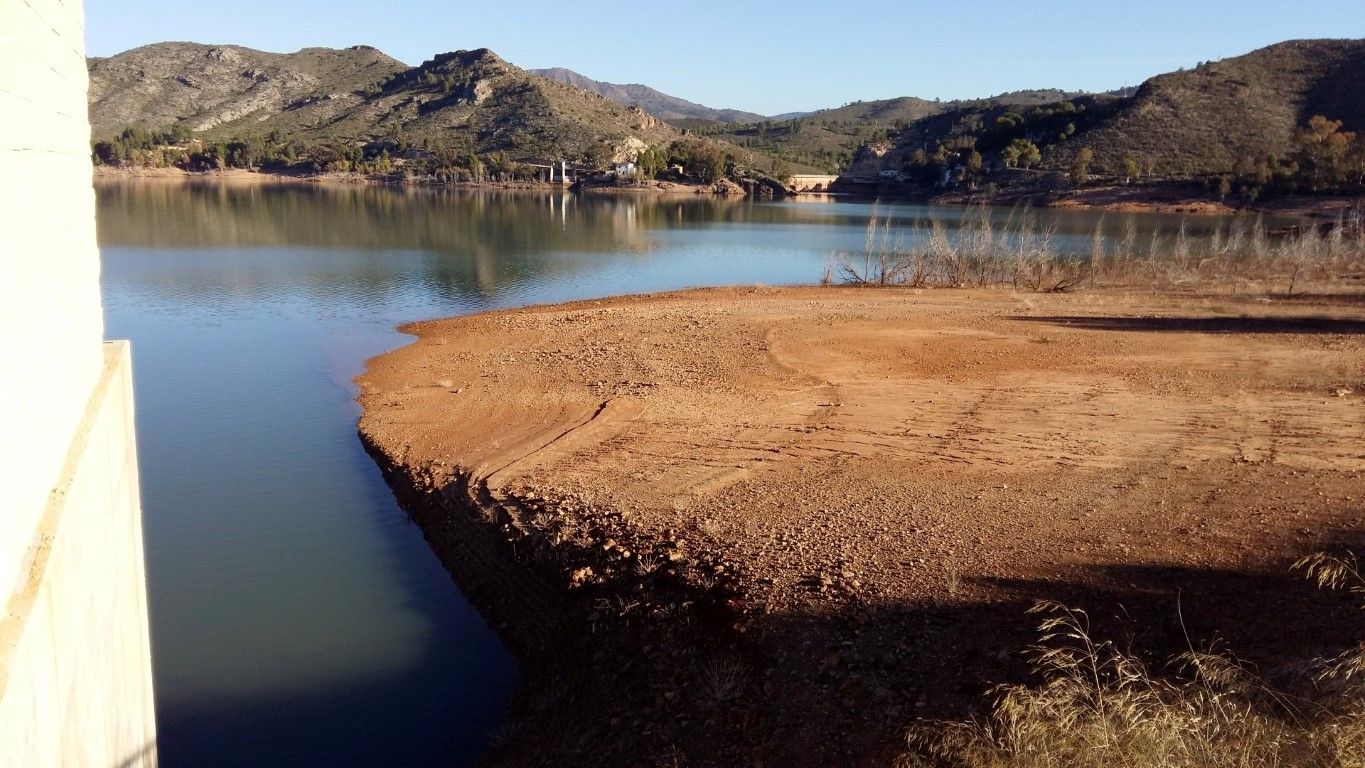
\includegraphics[width=0.3\linewidth]{imag/20151118_095151}
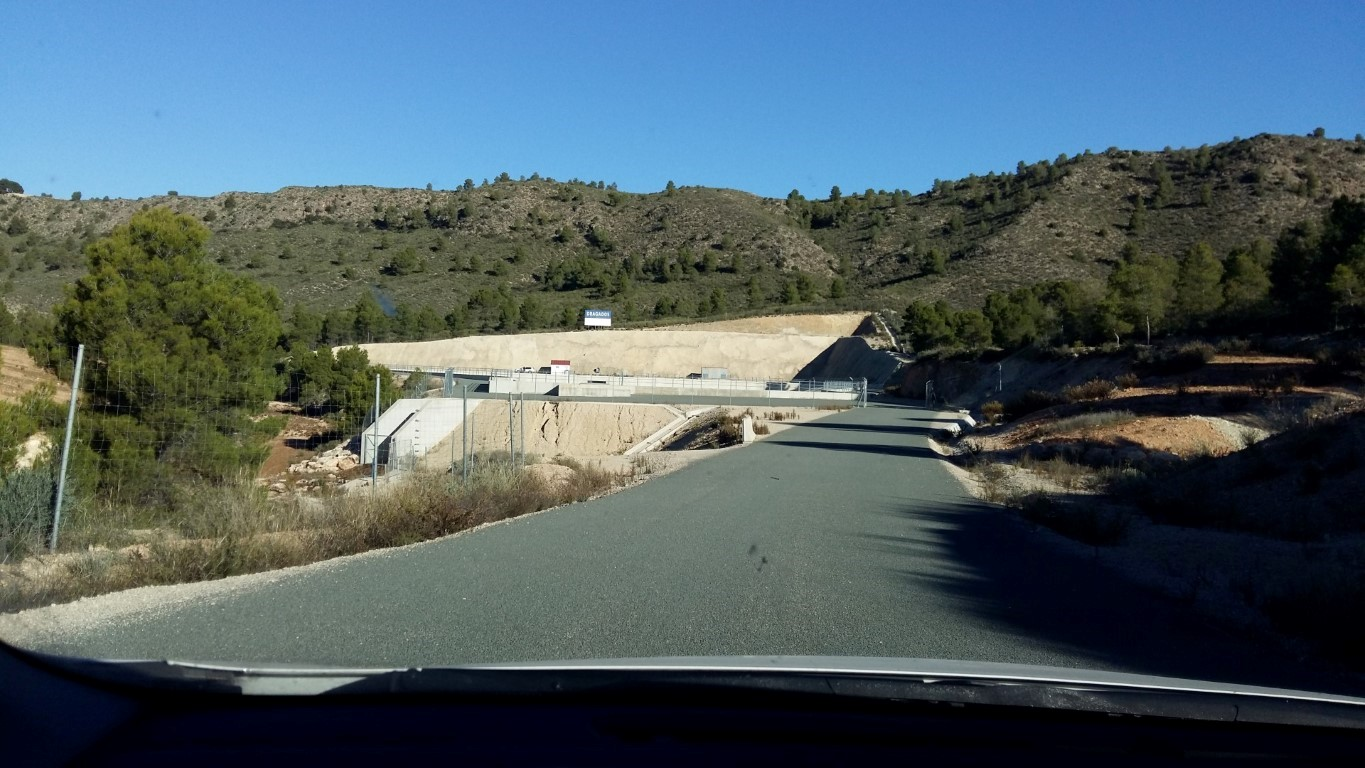
\includegraphics[width=0.3\linewidth]{imag/20151118_102505}
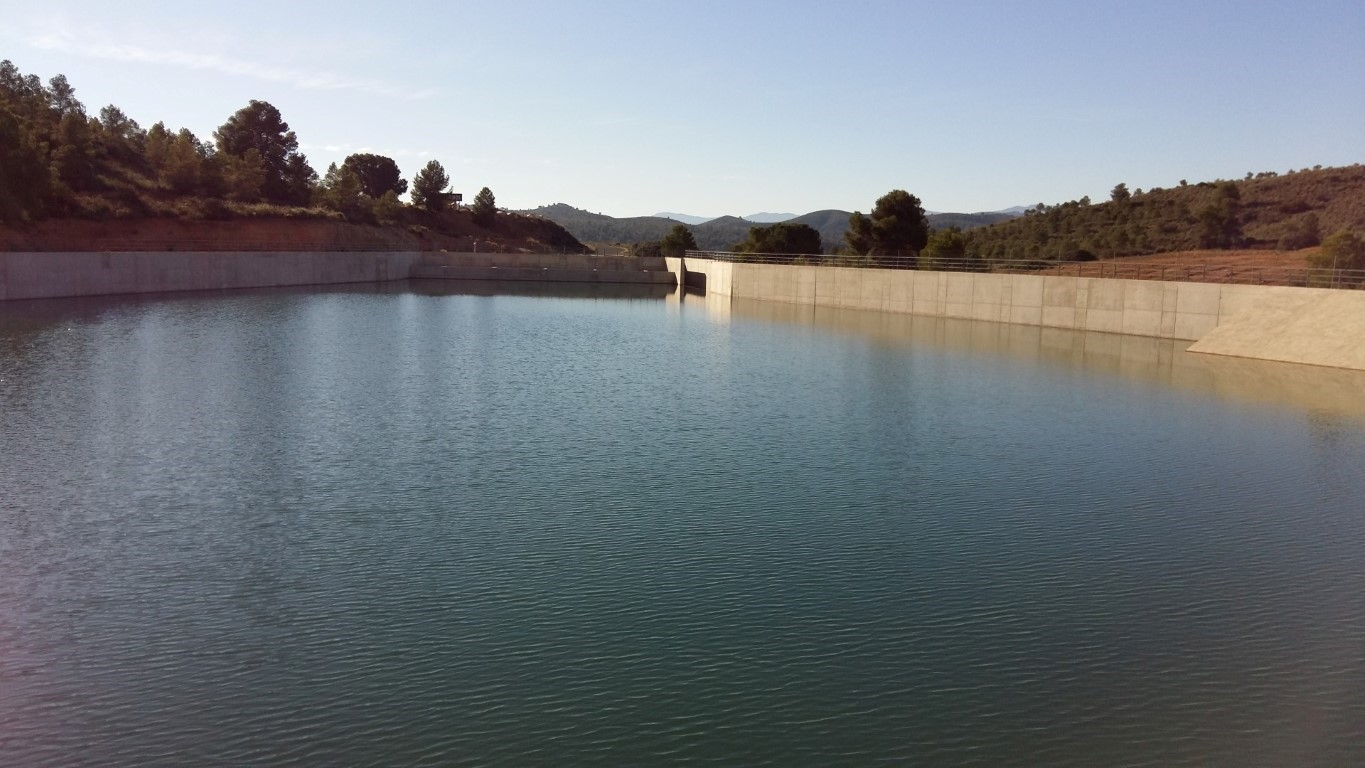
\includegraphics[width=0.3\linewidth]{imag/20151118_102617}
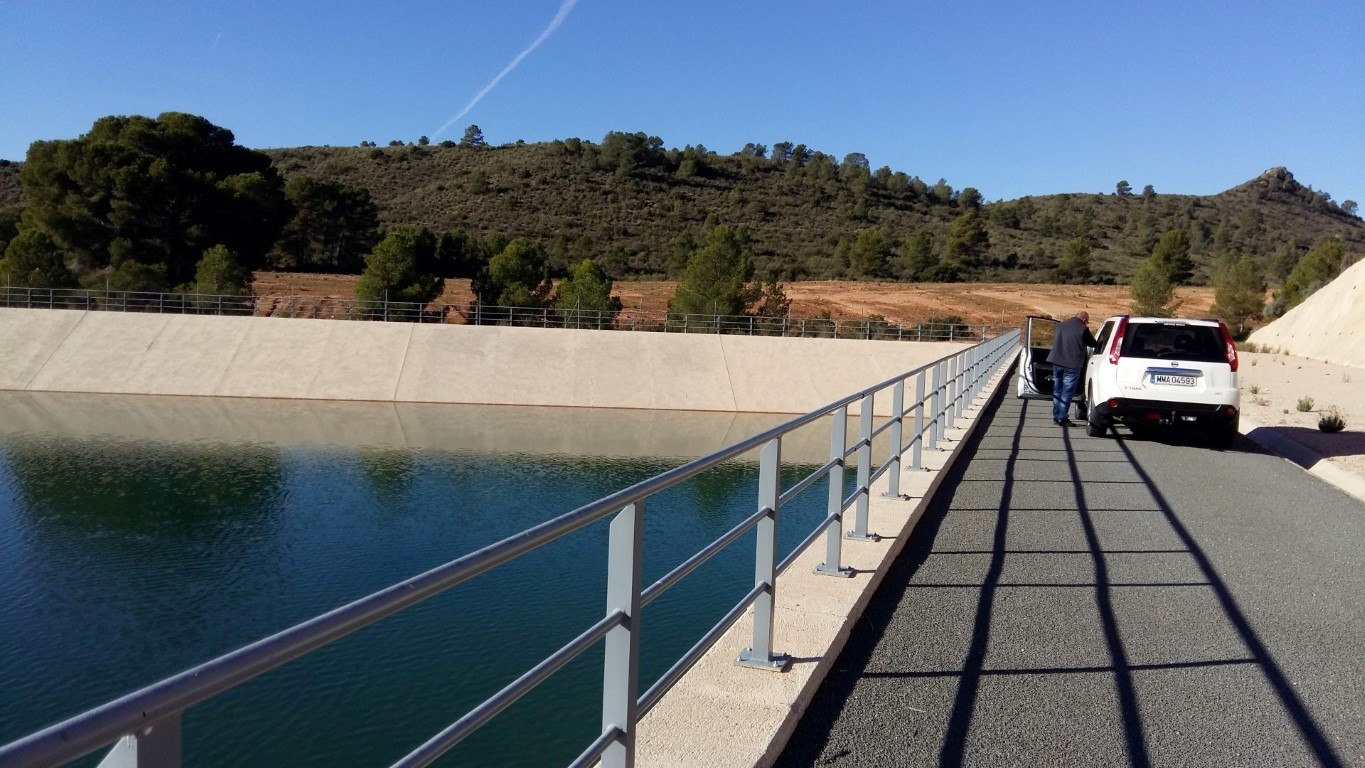
\includegraphics[width=0.3\linewidth]{imag/20151118_102621}
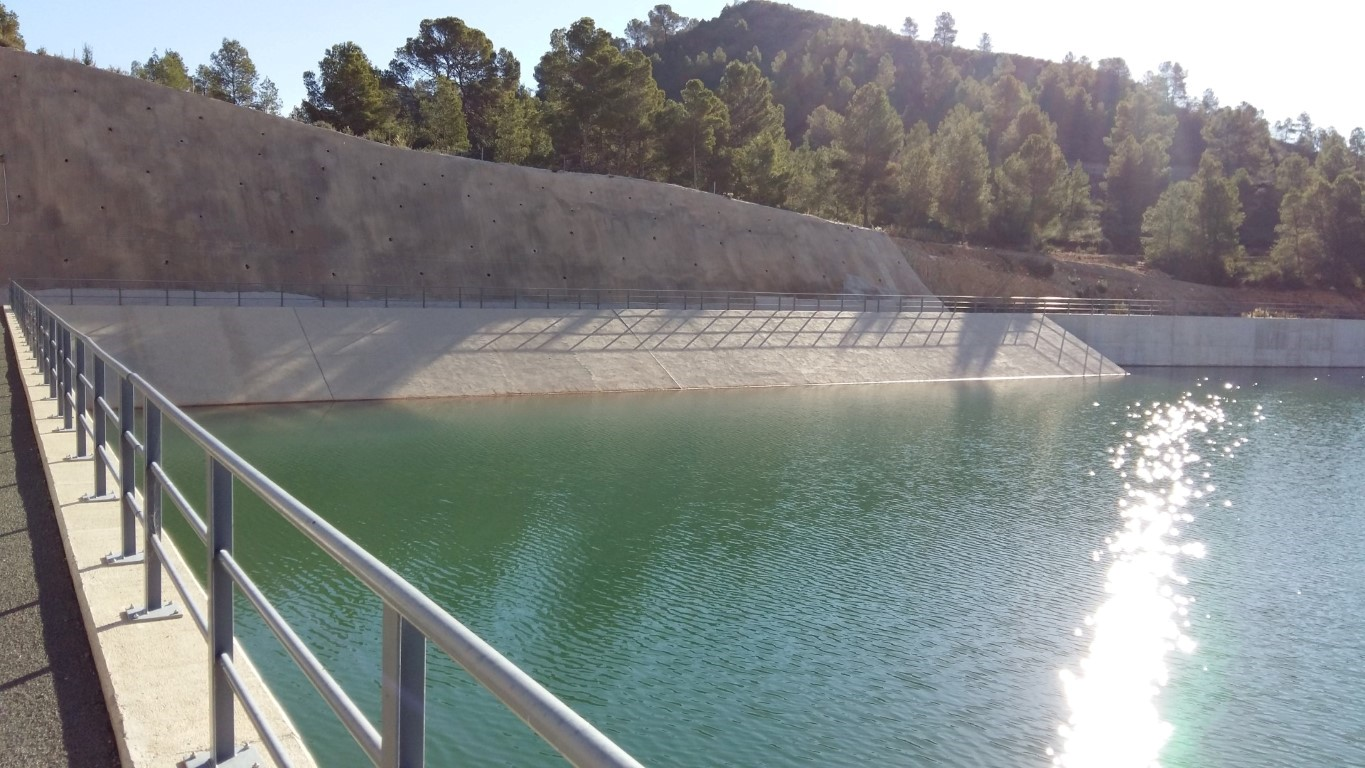
\includegraphics[width=0.3\linewidth]{imag/20151118_102626}
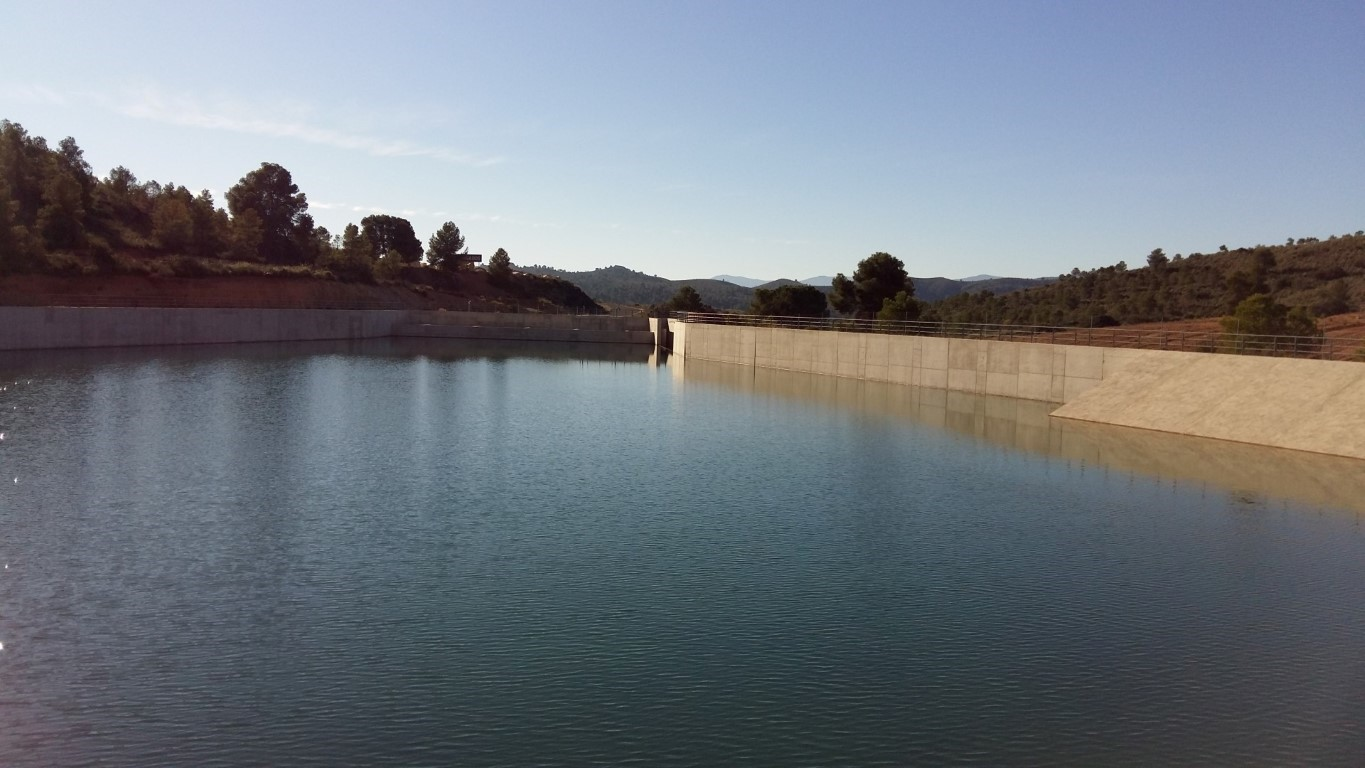
\includegraphics[width=0.3\linewidth]{imag/20151118_102710}
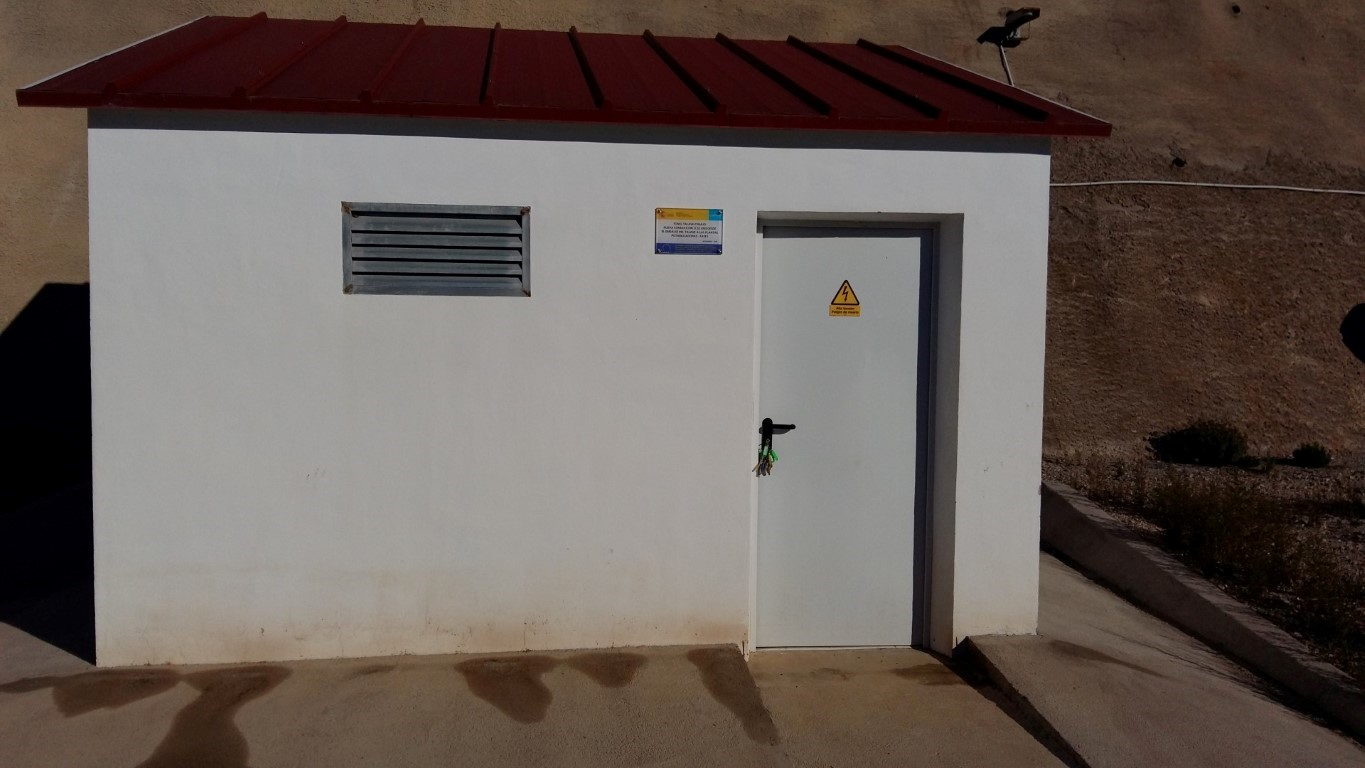
\includegraphics[width=0.3\linewidth]{imag/20151118_102928}
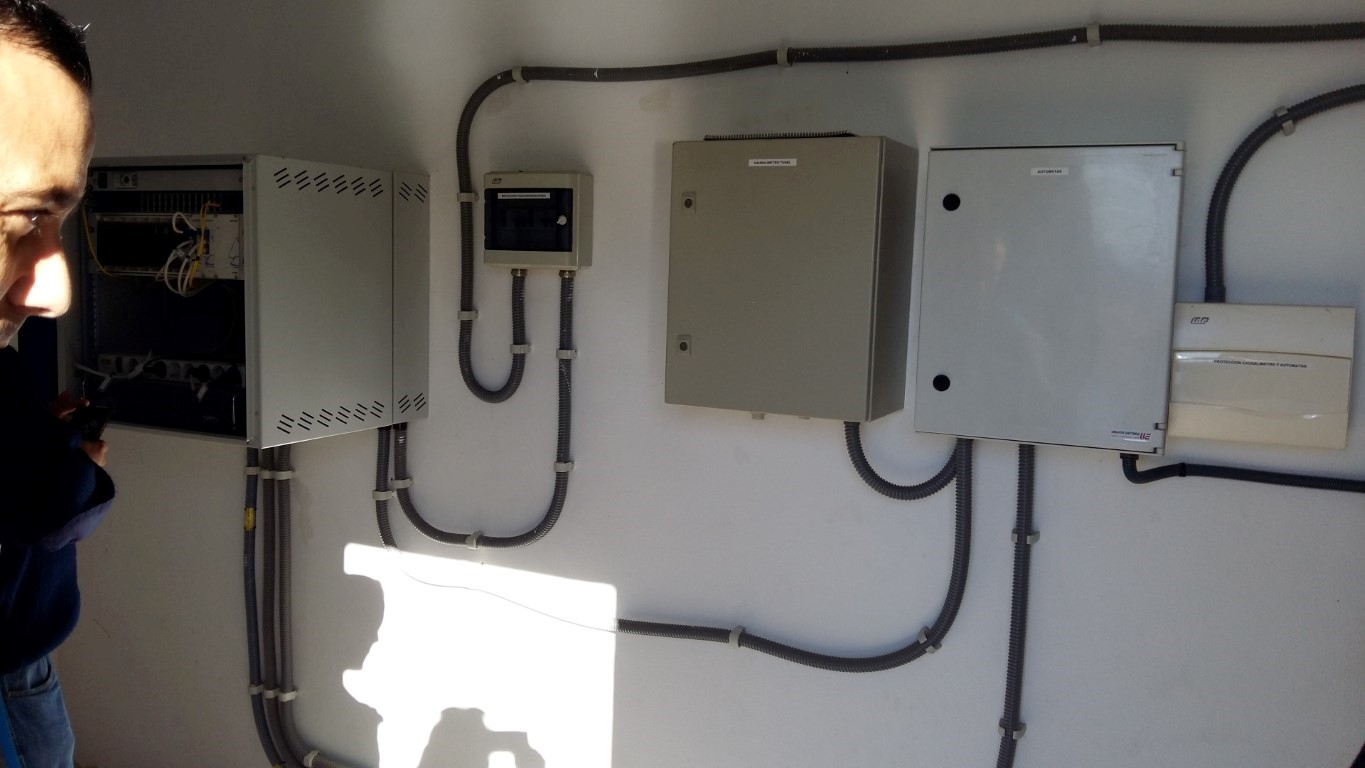
\includegraphics[width=0.3\linewidth]{imag/20151118_103019}
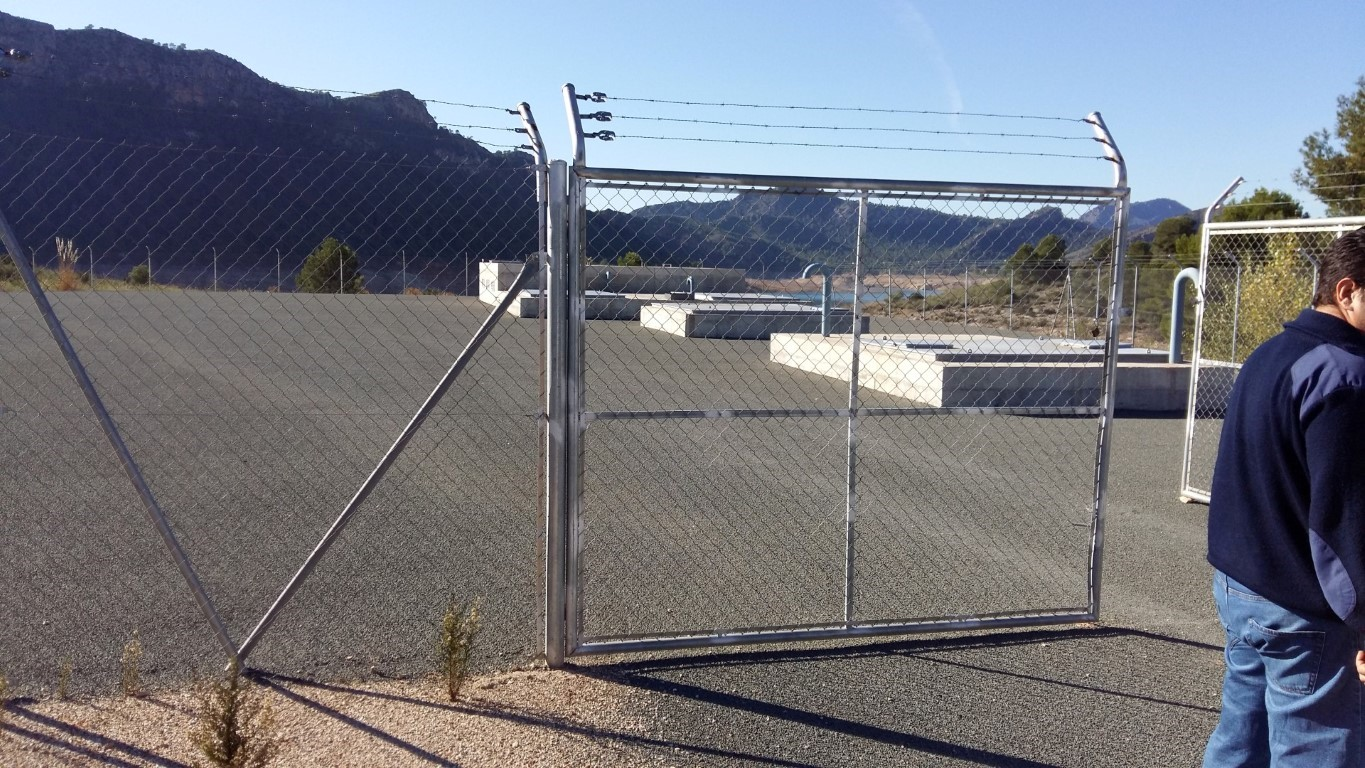
\includegraphics[width=0.3\linewidth]{imag/20151118_104655}
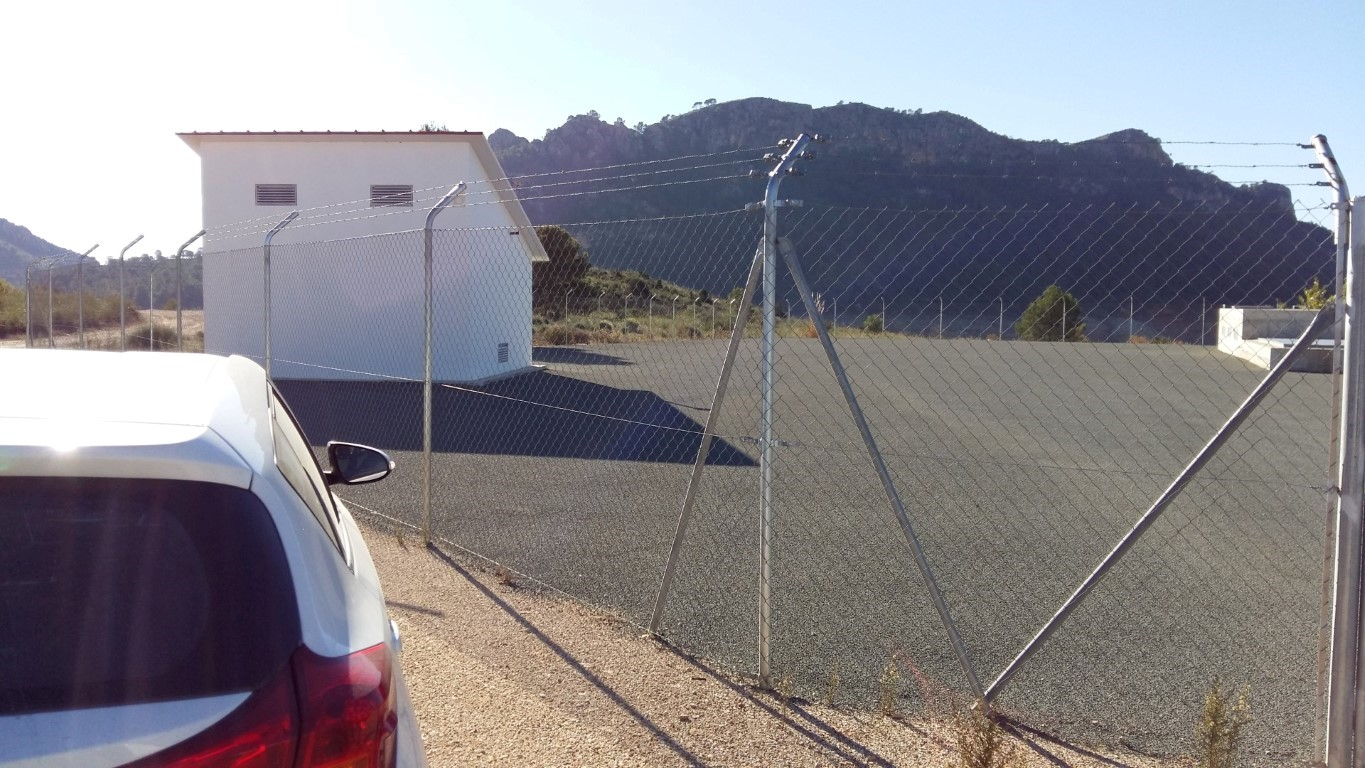
\includegraphics[width=0.3\linewidth]{imag/20151118_104658}
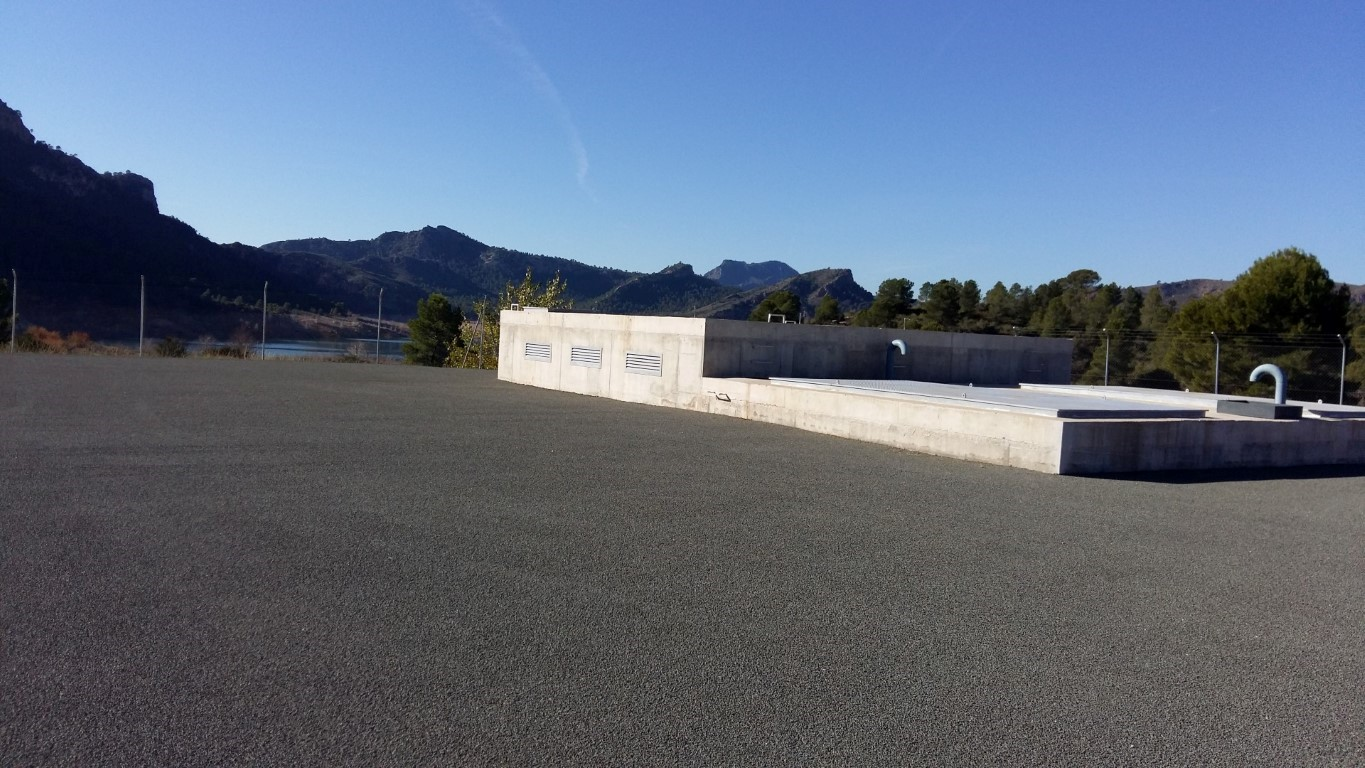
\includegraphics[width=0.3\linewidth]{imag/20151118_104736}
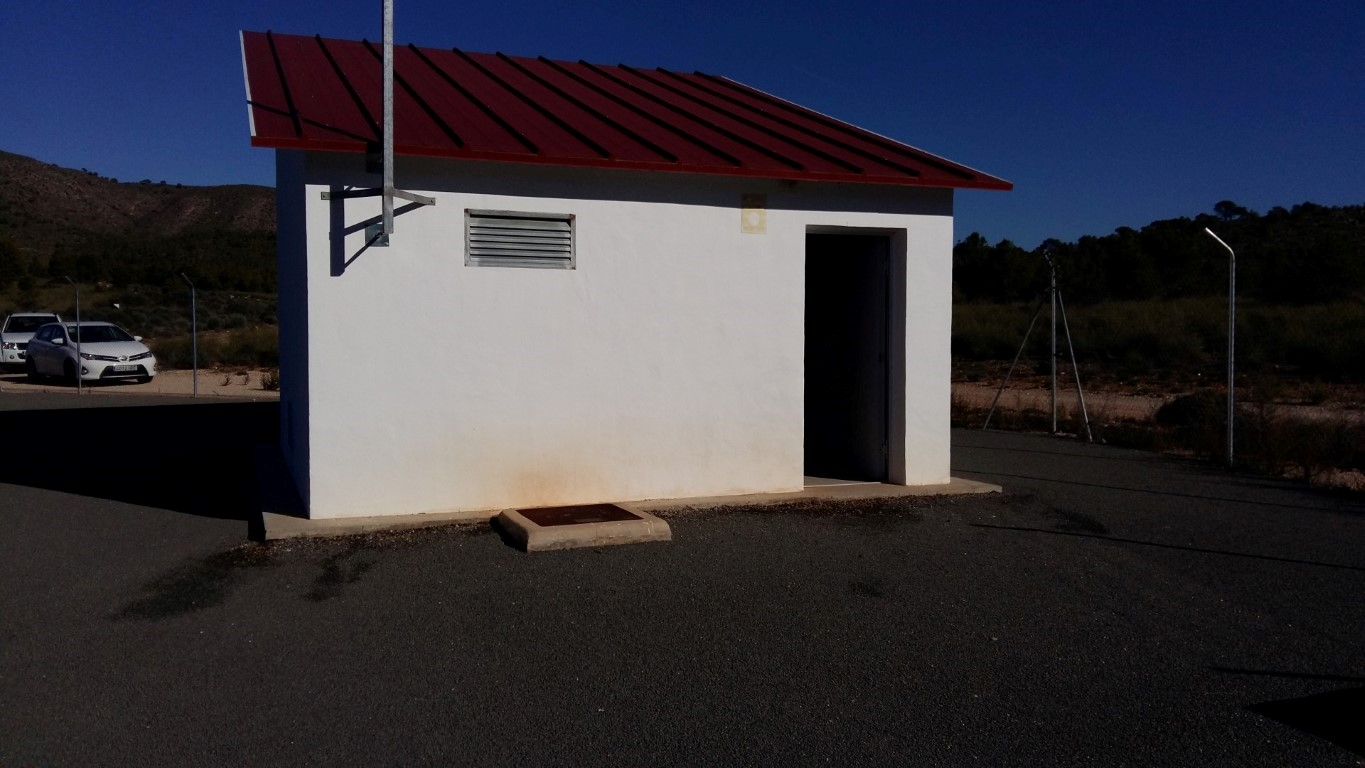
\includegraphics[width=0.3\linewidth]{imag/20151118_104811}
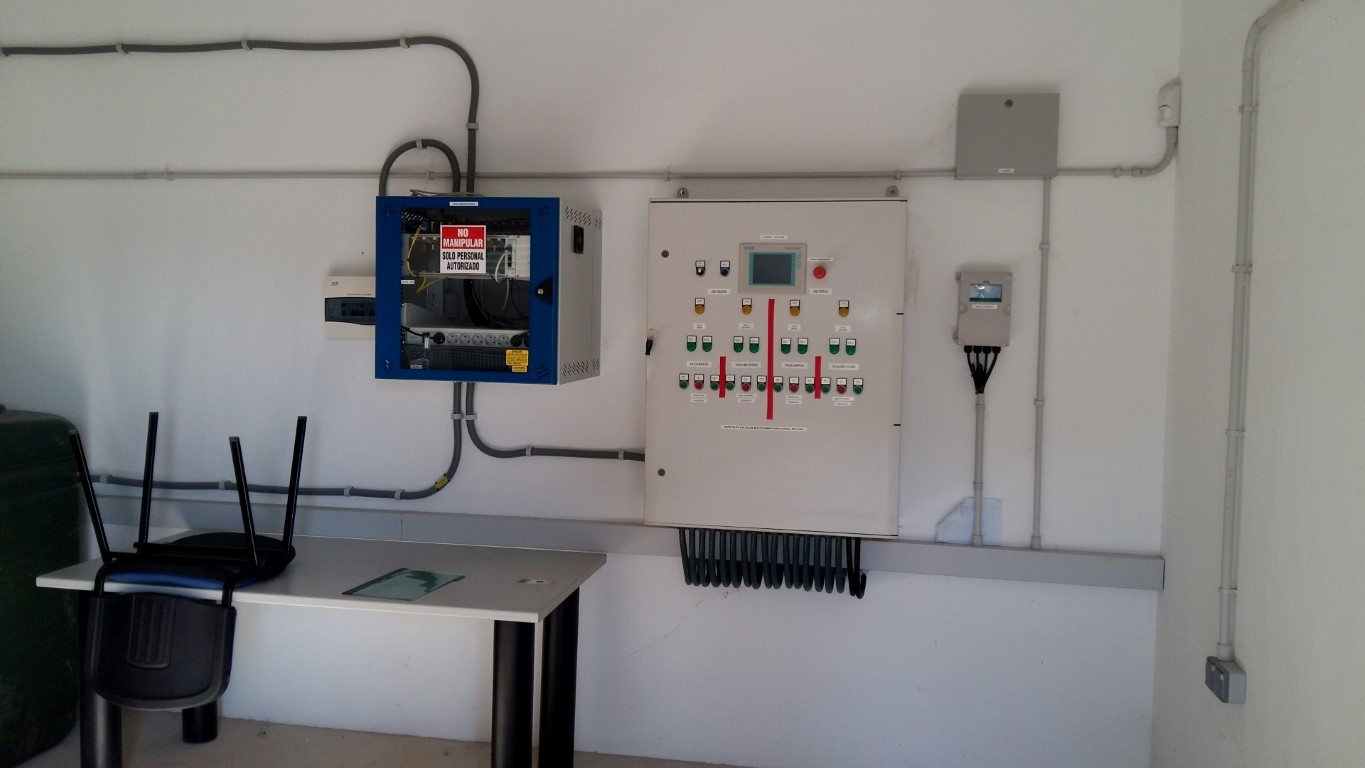
\includegraphics[width=0.3\linewidth]{imag/20151118_104830}

\section{REFERENCIAS}\label{referencias}

\bibliography{packages,libros}


\end{document}
